\section{Initial Data Processing}
\label{section:initial_processing}

The next phase was to extract the individual elements from each question and answers combination. The questions and answers from 57 users were downloaded with each users data stored in a single HTML file. To extract the data from these files Python and the Beautiful Soup HTML parsing library were used. After extracting the data from each file, it was written to a table in a MySQL database. The entire process can be summarised as shown in Figure \ref{fig:chapter4:extract_data_from_html}.

\begin{figure}[htbp]
	\centering
	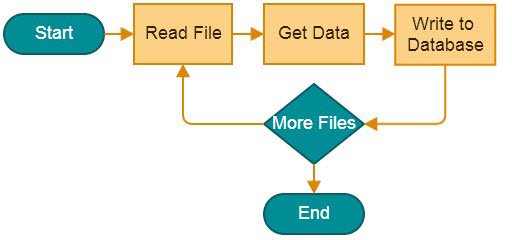
\includegraphics[width=0.5\textwidth]{Figures/Chapter4/extract_data_from_html.jpg}
	\caption[Simple process flow to extract data from HTML files]{Simple process flow to extract data from the HTML files downloaded from the Ask.fm website.}
	\label{fig:chapter4:extract_data_from_html}
\end{figure}

\subsection{Extract data from HTML Files}

Access to each HTML file is done using the glob and os packages. Each file is then parsed using the Beautiful Soup HTML parser (line 38). The script used to extract the data from the raw HTML files is included in Appendix \ref{app:parse_raw_data}. 

The individual data elements associated with each question and answer combination are contained within a HTML division element with a class attribute of \textit{``questionBox''}. A sample question box element is shown in Listing \ref{lst:chapter4.2:snipet_02}:

\begin{lstlisting}[language=html,caption={Sample question and answer HTML},label=lst:chapter4.2:snipet_02]
<div class='questionBox' id='question_box_107612243263'>
 <div class='question' dir='ltr'>
  <span>
   <span>I miss you</span>
  </span>
  <span class='author nowrap'>
   <a href='http://ask.fm/askerid'>
    askername
   </a>
  </span>
 </div>
 <div class='reportFlagBox '>
  <a href='http://ask.fm/userid/questions/107612243263'/>
 </div>
 <div class='answer' dir='ltr'>
  Text me?
 </div>
 <div class='time'>
  <a href='http://ask.fm/userid/answer/107612243263'>
   about 1 month ago
  </a>
 </div>
 <div class='likeList people-like-block'>
  <a href='http://ask.fm/likes/userid/question/107612243263' 
   1 person
  </a> likes this
 </div>
</div>
\end{lstlisting}

These data elements are examined in further detail later in this paper.

It is worth considering further the python in Appendix \ref{app:parse_raw_data} to understand how the data is extracted from the HTML files. As previously mentioned, each HTML file was parsed using the beautiful soup package resulting in an object called \verb|soup| that encapsulated all the file contents. From an earlier examination of the HTML it was known that each block of data was contained in a HTML division element that had a class attribute with a value of \verb|questionBox|. Line 55 shows how the \verb|soup.findAll()| method is applied to find all \verb|div| elements with a \verb|class| attribute with a value of \verb|questionBox| creating a list containing all question objects. Each question object is then individually retrieved for processing.

\begin{lstlisting}[firstnumber=55]
for a_question in soup.findAll("div", {"class": "questionBox"}):
\end{lstlisting}

Each of the seven data elements can then be extracted from this question object. Taking the question id first,  it is extracted from the \verb|id| attribute of the root question box division element. The value of the id attribute is split on the \verb|_| character and the question id is the third element of the array resulting from the split. In the sample HTML shown in Listing \ref{lst:chapter4.2:snipet_02} the question id is \verb|107612243263|. The python for this is shown on line 63. The \verb|strip| method simply removes any leading or trailing whitespace characters that may have been included in the extracted string.

\begin{lstlisting}[firstnumber=63]
question_id = a_question["id"].split("_")[2].strip()
\end{lstlisting}

The identification of the asker of the question and the number of likes that the question and answer have received are two more complicated examples because values for these elements may not exist so a check must be first performed to ascertain if the elements exist or not. To do this, a \verb|try| block is used. Taking the identification of the asker of the question as an example, the \verb|find| method is used on the question object to search for an element that has an \verb|author nowrap| attribute with a child \verb|a| element. If so then the asker identification is in contained in the \verb|href| attribute. As the value of this attribute is a URL the string is split on the \verb|/| character with the fourth value of the resulting array containing the required value. If the required elements do not exist in the question object, that is the question was asked anonymously, an exception is caught and the data element is set to an empty value:

\begin{lstlisting}[firstnumber=78]
try:
	if a_question.find(attrs="author nowrap").			\
	 	a["href"].split("/")[3]:
	  ask_id = a_question.find(attrs="author nowrap").	\
	  a["href"].split("/")[3].strip()
except (AttributeError, KeyError):
	ask_id = ""
\end{lstlisting}

The final step is to write the data extracted from the HTML files to a database. For this purpose a MySQL database called \verb|thesis| was created as well as a table called \verb|raw_data| to house the question and answer data elements. In the Python script the first step is to create a database connection and then using this connection create a cursor object. When the data elements for each question and answer block have been extracted the required SQL code is then executed to write the data to the database. All database related code is executed with a try block in case an exception is thrown. In Appendix \ref{app:parse_raw_data} lines 41 - 50 show where the database connection is created and lines 105 - 124 where each record extracted is written to the database. This is just a brief summary of some of the main functionality of the python script used. Other functionality not discussed includes making the users identification and the question number anonymous.

\subsection{Splitting the data}

The final part of the initial processing performed on the data was to split the 109,312 samples into three blocks of data. It was decided to divide the dataset into blocks of 10\% for initial classification, model training and test, 80\% to later simulate a stream of data arriving at the Ask.fm website and the final 10\% for validation purposes. The details of how the block of 80\% of the data and the second 10\% validation block will be explained later.

Before splitting the dataset, it was decided that the only criteria imposed would be that the proportions of questions per user should be maintained. For example, if user \verb|X| has 2,400 questions, after the split this user would have approximately 240 questions in the first block, 1,920 in the second block and 240 in the third. 

Although there are many ways to split data in the manner required, called stratified sampling, it was decided to use IBM SPSS Modeler. The model used is shown in Figure \ref{fig:chapter4:data_partitioning}.

\begin{figure}[htbp]
	\centering
	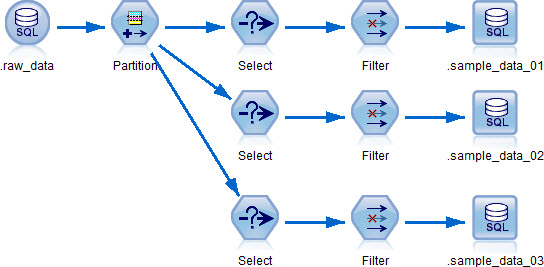
\includegraphics[width=0.75\textwidth]{Figures/Chapter4/data_partitioning.jpg}
	\caption[Partitioning data using IBM SPSS]{IBM SPSS Modeler process to split the dataset into three groups.}
	\label{fig:chapter4:data_partitioning}
\end{figure}

Using a \verb|SQL| operator a connection is created to the database and the raw data is extracted. It should be noted that this operator uses an ODBC connection to the database that must be created is advance. A \verb|Partition| operator is then used to split the data as required on the anonymous user id. The details of this operator are shown in Figure \ref{fig:chapter4:partition_operator}. The required split into three groups, based on the anonymous user identification field \verb|u_id| field, can be clearly seen. In the Figure \ref{fig:chapter4:partition_operator} it can also be seen that a new partition attribute is added to the data to help identify which group each record belongs to. This new attribute will be used in the next operator to split the data into the three required groups. 

\begin{figure}[htbp]
	\centering
	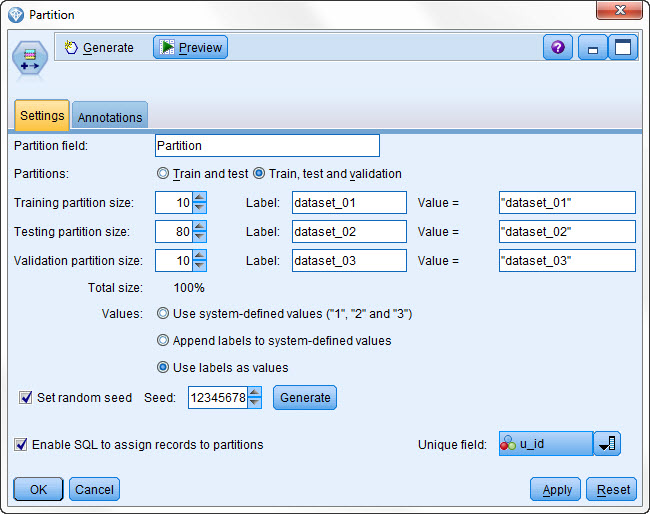
\includegraphics[width=0.75\textwidth]{Figures/Chapter4/partition_operator.jpg}
	\caption[Partition operator used generate a new attribute]{The Partition operator that is used generate a new partition attribute on which the data will be split.}
	\label{fig:chapter4:partition_operator}
\end{figure}

The output of the \verb|Partition| operator is then used as input into three separate \verb|Select| operators. The input to each of these operators is the same, the complete dataset, but as can be seen in Figure \ref{fig:chapter4:select_filter} only records that match the given condition, in this case \verb|Partition = "dataset_01"|, are passed through to the next operator which is the \verb|Filter| operator. Although it would be possible at this point to write the entire record of the question to the database, this would represent significant data repetition and redundancy. Using views in the database means that it is only necessary to write the anonymous question id of each record to the database. Once the question id is know then it will be possible to access any other attributes or columns as required using SQL. Only the anonymous question id, \verb|q_id|, is allowed pass through to the final operator where the anonymous question ids of the three blocks of data are each written to their respective tables created solely for this purpose.

\begin{figure}[htbp]
	\centering
	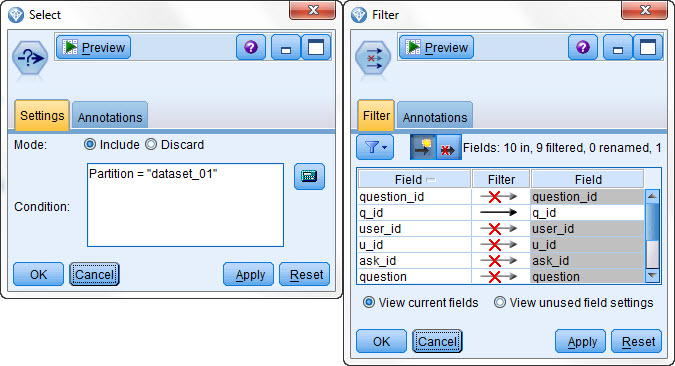
\includegraphics[width=0.75\textwidth]{Figures/Chapter4/select_filter.jpg}
	\caption[Select operator and the Filter operator settings]{The Select operator and the Filter operator settings.}
	\label{fig:chapter4:select_filter}
\end{figure}

Further details about the format, structure and contents of the data and the database housing the data at this point in the process is provided in the Section \ref{section:data_exploration}.

